\chapter{Solar flare detection}

Before starting to develop the main solar flare detection algorithm a first program was developed that would target a powerful solar flare for which we knew the time of the event and therefore, the location of the Sun.

Although the aim of the main algorithm is detecting the solar flare without taking into consideration the position of the Sun, this first approach was done to understand how the inner part of the algorithm works: studying the correlation between the cosine of the solar-zenith angle and the VTEC content.

This sections also provides an introduction to the formatting and use of the Global Navigation Satellite Systems data (GPS in this case) and how the main parameters necessary for the algorithms are computed.

\section{Data}

\subsection{GPS Data}

As we have seen in previous sections, the International GNSS Service (IGS) has made available open access GNSS data since its creation. The Crustal Dynamics Data Information System (CDDIS) is a central data archive for the NASA's Crustal Dynamics Project (CDP). This archive has supported the IGS since 1992 by storing and providing access to the GNSS data generated by the IGS.

Figure \ref{fig:exampleCDDIS} shows how data is stored in de CDDIS server (\url{ftp://cddis.nasa.gov/gps/data/hourly/}).

The files in this server contain raw GPS data that is then pre-processed to obtain VTEC maps in the form of \textbf{ti} files. An example diagram of this complex, several step process is shown in figure \ref{fig:diagramIGS}, extracted from the paper "The IGS VTEC maps: a reliable source of ionospheric information since 1998" \cite{hernandez2009igs} by Manuel Hernández-Pajares, which offers a detailed explanation of this process. 

\begin{figure}[!htb]
	\begin{subfigure}[b]{0.3\textwidth}
		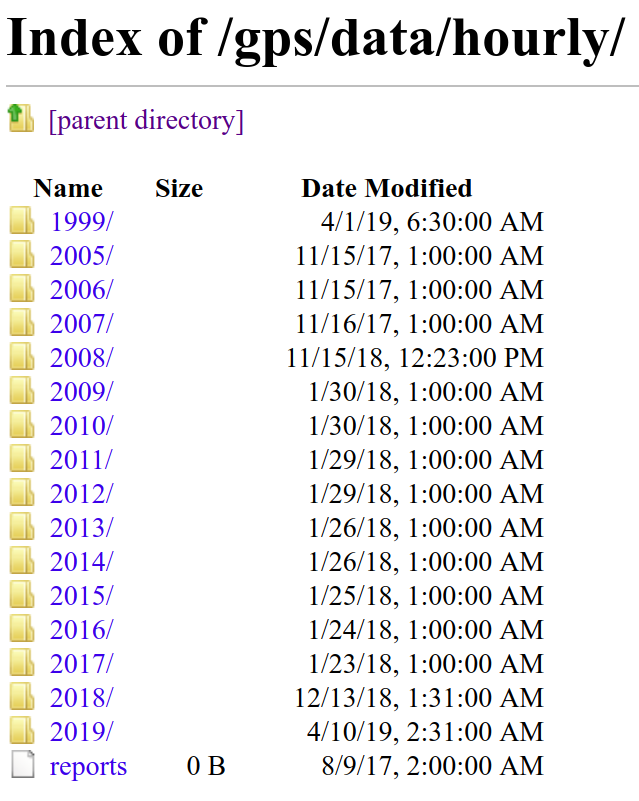
\includegraphics[width=\linewidth]{images/ch4/FTPNASA.png}
		\caption{Files}
	\end{subfigure}
	\hfill
	\begin{subfigure}[b]{0.5\textwidth}
		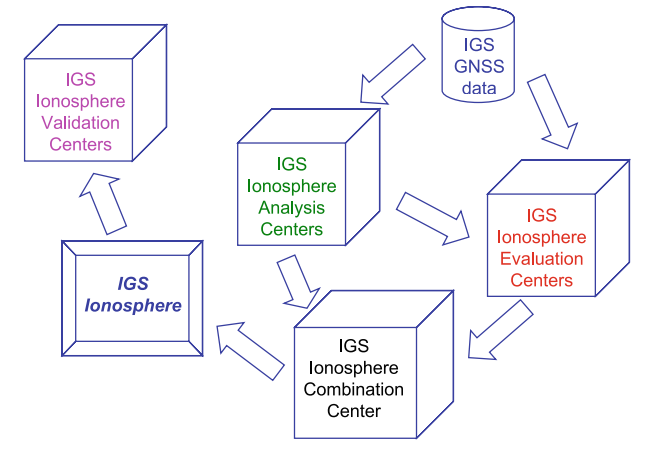
\includegraphics[width=\linewidth]{images/ch4/DataFlowIGS.png}
		\caption{Data flow}
	\end{subfigure}
	\caption{VTEC distribution throughout the day for all IPPS (a) and for IPPs that have Vill as the receiver (b)}
	\label{fig:exampleCDDIS}
\end{figure}


However, for this and the following section, only the pre-processed ti files of past dates were needed, as detecting the flares in real time is a task that will be discussed later in the project, in which this pre-processing will have to be taken into consideration. The project supervisor, Manuel Hernández-Pajares, provided me with some of these maps to use as input data for the algorithms, along with information about the formatting of this files.

% \cite{cddisnasa} -> The Crustal Dynamics Data Information System (CDDIS) was initially developed to provide a central data bank for NASA's Crustal Dynamics Project (CDP). The system continues to support the space geodesy and geodynamics community through NASA's Space Geodesy Project as well as NASA's Earth Science Enterprise. The CDDIS was established in 1982 as a dedicated data bank to archive and distribute space geodesy related data sets. Today, the CDDIS archives and distributes mainly Global Navigation Satellite Systems (GNSS, currently Global Positioning System GPS and GLObal NAvigation Satellite System GLONASS), laser ranging (both to artificial satellites, SLR, and lunar, LLR), Very Long Baseline Interferometry (VLBI), and Doppler Orbitography and Radio-positioning Integrated by Satellite (DORIS) data for an ever increasing user community of geophysists.
% The CDDIS is operational on a dedicated computer located at the Goddard Space Flight Center in Greenbelt, MD.
% The CDDIS has served as a global data center for the International GNSS Service (IGS) since 1992. The CDDIS also actively supports the International Laser Ranging Service (ILRS), the International VLBI Service for Geodesy and Astrometry (IVS), International DORIS Service (IDS), and the International Earth Rotation and Reference Systems Service (IERS) as a global data center.
% To learn more about these space geodetic techniques and their respective CDDIS data holdings, click on the images below.

% \cite{noll2010crustal} -> Since 1982, the Crustal Dynamics Data Information System (CDDIS) has supported the archive and distribution of geodetic data products acquired by the National Aeronautics and Space Administration (NASA) as well as national and international programs. The CDDIS provides easy, timely, and reliable access to a variety of data sets, products, and information about these data. These measurements, obtained from a global network of nearly 650 instruments at more than 400 distinct sites, include DORIS (Doppler Orbitography and Radiopositioning Integrated by Satellite), GNSS (Global Navigation Satellite System), SLR and LLR (Satellite and Lunar Laser Ranging), and VLBI (Very Long Baseline Interferometry). The CDDIS data system and its archive have become increasingly important to many national and international science communities, particularly several of the operational services within the International Association of Geodesy (IAG) and its observing system the Global Geodetic Observing System (GGOS), including the International DORIS Service (IDS), the International GNSS Service (IGS), the International Laser Ranging Service (ILRS), the International VLBI Service for Geodesy and Astrometry (IVS), and the International Earth rotation and Reference frame Service (IERS). Investigations resulting from the data and products available through the CDDIS support research in many aspects of Earth system science and global change. Each month, the CDDIS archives more than one million data and derived product files totaling over 90 Gbytes in volume. In turn, the global user community downloads nearly 1.2 Tbytes (over 10.5 million files) of data and products from the CDDIS each month. The requirements of analysts have evolved since the start of the CDDIS; the specialized nature of the system accommodates the enhancements required to support diverse data sets and user needs. This paper discusses the CDDIS, including background information about the system and its user communities, archive contents, available metadata, and future plans.

\subsection{Formatting}

The ti files contain several rows of pre-processed GPS data. Each row has a Receiver Id. and a Transmitter Id., therefore, for each row we have an Ionospheric Piercing Point (IPP), that has been presented before in the backround section, the TODO: definicion correcta de IPP.

For each of these rows/IPPs, several parameters are relevant for our computations:


\begin{itemize}
\item The \textbf{GPS time}
\item The \textbf{Receiver Id.}
\item The \textbf{Transmitter Id.}
\item The \textbf{double derivate of LI} (d2li) TODO: explicar bien esto
\item The \textbf{xmappingion} function, TODO: este tambien
\item The \textbf{right ascension} and \textbf{declination} of the IPP
\end{itemize}

\begin{lstlisting}[caption=Format of the ti file]
Field number | Example value | Description
[...]
3 		0.008333333333		GPS time/hours (tsecdayobs/3600.d0)
4 		cand							Receiver Id.
5 		3									Transmitter Id.
[...]
21 		-0.5131586E-02		d2li
[...]
43 		0.1565765332E+01		xmapping_ion
44 		334.449							xraion
45 		33.092							xlation
[...]
\end{lstlisting}

\subsection{The Halloween Solar Storm: X17.2 flare}

The data set we used was that of so-called Halloween Storm, a powerful solar storm that took place from October to early November. In particular, we will try to replicate the results shown in figure \ref{fig:halloweenPaper}, obtained in the paper "GNSS measurement of EUV photons flux rate during strong and mid solar flares" for a poweful flare that took place in October 28th, 2003 \cite{hernandez2012gnss}.

\begin{figure}[!htb]
	\begin{centering}
		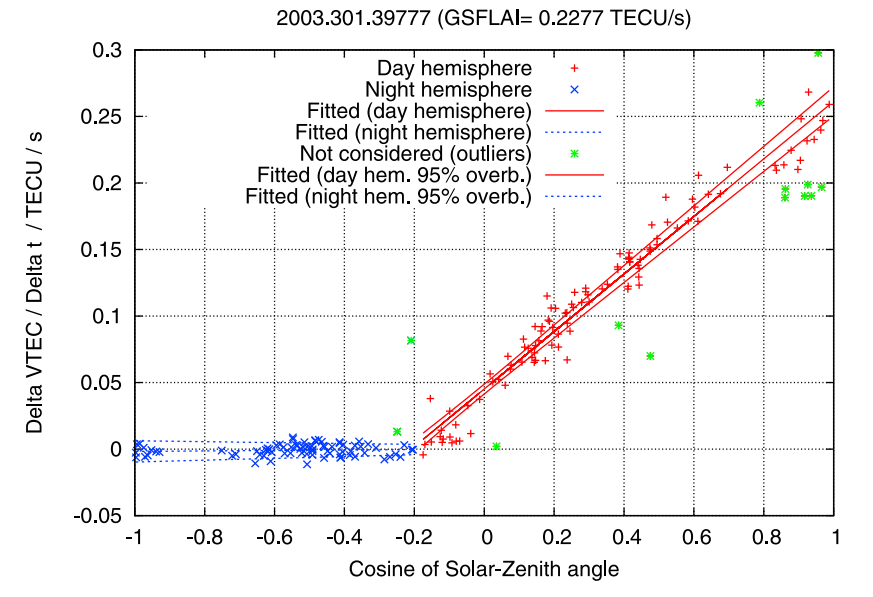
\includegraphics[width=0.5\linewidth]{images/ch4/halloweenPaper.png}
		\caption{VTEC distribution throughout the day for all IPPS (a) and for IPPs that have Vill as the receiver (b)}
		\label{fig:halloweenPaper}
	\end{centering}
\end{figure}

As we can see the plot of the flare called X17.2 took place exactly at 2003.301.39777 (year.day.seconds of GPS time). In hours, 39777 seconds of a day is $39777s * 1h/3600s = 11.049...h$, around 11AM. 

The ti files provided contained data from 10.5h to 11.5h (with a sampling rate of 30 seconds), so that we could see the VTEC distribution through the day.

With this data we can obtain the two parameters that will yield the plot shown in figure \ref{fig:halloweenPaper}: the \textbf{VTEC value} and the \textbf{cosine of the solar-zenith angle}.

\section{VTEC}

Fisrt we wanted to obtain VTEC distribution throughout the day, to visually see if any spikes appeared confirming that the moment we were going to study based on the paper \cite{hernandez2012gnss} was correct.

For each epoch in our data set (from 10.5 to 11.5 with a sampling rate of 30 seconds) we needed to compute de VTEC value.

\subsection{Computing the VTEC}

As we have mentioned before, one of the main paramenters relevant to the computation is the \textbf{double derivate of LI (d2li)}. Because this is a derivative it is the increment in VTEC, this will be seen in a moment in figure \ref{fig:vtecDistribution}.

The VTEC can be estimated using the following approach:

\begin{equation} \label{eq:1}
	\frac{d^{2}V}{dt^{2}} = \frac{d^{2}Li}{M}
\end{equation}

Where $M=\frac{1}{\cos Z}$ is the "ionospheric mapping function", given by the inverted cosine of the satellite-zenith angle that we have for each IPP. \cite{hernandez2012gnss}

Therefore, we can estimate the VTEC of an IPP by dividing two of the given fields in the data file:
\begin{equation} \label{eq:2}
	VTEC \approx \frac{d^{2}Li}{M}
\end{equation}
The Vtec...formulas...d2li/mappingio


\subsection{Distribution throughout the day}

Because the only operation that had to be performed was the previous division, a simple AWK script was used to filter out the two necessary fields from the data file (d2li and  mapping) and print the resulting value and the time. 

\begin{lstlisting}[language=Awk, caption=process]
{
	/a/
	d2li = $21;
	mappingFunc = $43;
	vtec = d2li/mappingFunc;
	print $3 " " vtec
}
\end{lstlisting}

\begin{lstlisting}[language=Bash, caption=Bash script to execute the procedures]
#!/bin/bash
tiDataFile="../data/ti.2003.301.10h30m-11h30m.gz"

zcat "$tiDataFile" | gawk -f previewVTECDistribution.awk > vtecValues
gnuplot -e "set terminal png; set output 'vtecDistribution.png'; set title 'VTEC Distribution'; set xlabel 'Time of the day (hours)'; set ylabel 'VTEC'; set grid; plot \"vtecValues\" using 1:2 with point"
rm vtecValues
\end{lstlisting}
\clearpage

The bash script executes the AWK process with the data as the input and outputs n rows with two columns: the time of the day and the calculated VTEC, plotting the results using Gnuplot.
The results can be seen in figure \ref{fig:vtecDistribution}, where we can see how the VTEC value evolves throught the day. Visually, a spike can be seen between 11 and 11.2 hours. 

As mentioned before this value is estimated using the derivative of li, because this is the increment in VTEC, we can see that the value becomes negative after the spike, due to the VTEC value decreasing (negative gain).

\begin{figure}[!htb]
	\begin{subfigure}[b]{0.5\textwidth}
		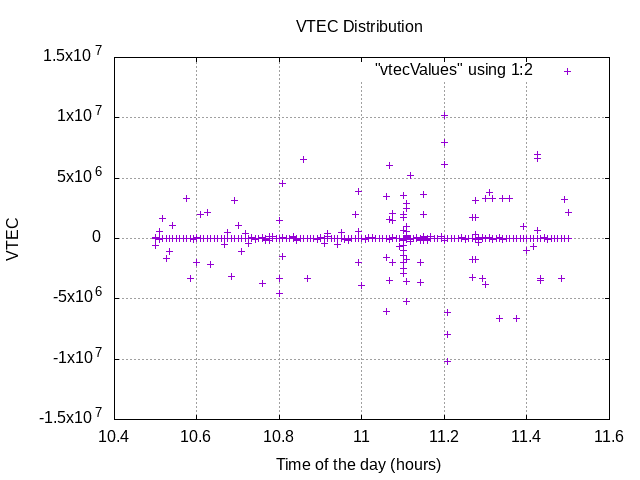
\includegraphics[width=\linewidth]{images/ch4/vtecDistributionGeneral.png}
		\caption{All IPPs}
	\end{subfigure}
	\hfill
	\begin{subfigure}[b]{0.5\textwidth}
		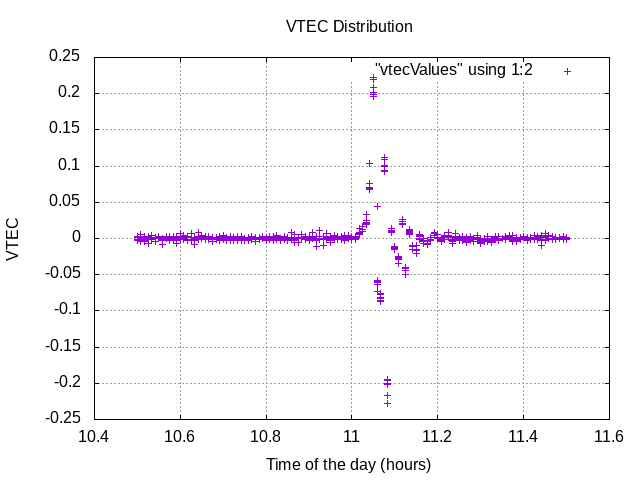
\includegraphics[width=\linewidth]{images/ch4/vtecDistributionVill.png}
		\caption{Villafranca station}
	\end{subfigure}
	\caption{VTEC distribution throughout the day for all IPPS (a) and for IPPs that have Vill as the receiver (b)}
	\label{fig:vtecDistribution}
\end{figure}

To see the event more clearly, though, we can focus on one specific receiver (which will still yield multiple IPPs, as the receiver works with different satellites). For the particular case of the Villafranca, Spain station (identified as Vill), we obtain the plot from figure \ref{fig:vtecDistribution}(b). At this time of the day around 11:00h the Sun would have a greater effect on the IPPs of this station, so the spike can be seen more clearly. 

As mentioned before, the flare took place at 11.05, so we could proceed using the studied data range and this epoch in particular.

\section{Solar-zenith angle}

The solar-zenith angle (denoted $\chi$ from now onward) plays a major role when studying this event: it is the angle formed by the Sun and the Earth's zenith and indicates the effect the flare is having on a particular IPP. It is expected that this variable presents a correlation with the increase in VTEC, which is what we aim to observe in this chapter.

Figure \ref{fig:solar-zenith-angle}, at the end of the chapter, provides a visual representation of this variable that along with the results depicts how it can affect the VTEC value. 

Obtaining the angle between two celestial objects has been shown in the previous section by means of equations \ref{eq:1}, \ref{eq:2} and \ref{eq:3}, when calculating the angle between the Sun and a detected GRB.

\begin{equation} \label{eq:1}
unitVectorObjectA =	
\begin{bmatrix}
\cos\delta_{g} * \cos\alpha_{g} \\ 
\cos\delta_{g} * \sin\alpha_{g} \\
\sin\delta_{g}
\end{bmatrix}
\end{equation}

\begin{equation} \label{eq:2}
unitVectorObjectB =	
\begin{bmatrix}
\cos\delta_{s} * \cos\alpha_{s} \\ 
\cos\delta_{s} * \sin\alpha_{s} \\
\sin\delta_{s}
\end{bmatrix}
\end{equation}

\begin{equation} \label{eq:3}
\cos \beta = unitVectorObjectA \cdot unitVectorObjectB
\end{equation}\\

For this case, though, the angle is computed using the IPP's Right Ascension and Latitude (equivalent to declination), yielding the cosine of $\chi$, the \textbf{solar-zenith angle}. The previous dot product can be simplified to:

\begin{equation} \label{eq:4}
\cos \chi = \sin\delta_{IPP}*\sin\delta_{Sun} + \cos\delta_{IPP}*\cos\delta_{Sun}*\cos(\alpha_{IPP} - \alpha_{Sun})
\end{equation}\\

The following code is the function that implements equation \ref{eq:4} and returns $\cos \chi$:

\begin{lstlisting}[language=Fortran, caption=Computation of the solar-zenith a angle's cosine]
real function computeSolarZenithAngle (raIPP, decIPP, raSun, decSun)
			implicit none

			real, intent(in) :: raIPP, decIPP, raSun, decSun
			real :: solarZenithAngle
			
			solarZenithAngle = sin(decIPP)*sin(decSun) + cos(decIPP)*cos(decSun)*cos(raIPP - raSun)
			return
		end function computeSolarZenithAngle
\end{lstlisting}

\section{Results}

Taking $212.338º$ and $-13.060º$ as the Sun's right ascension and declination, respectively, and the measurements of all IPPs at 11.05 hours, figure \ref{fig:results} shows the plot of the output of our program.

\begin{figure}[!htb]
\begin{centering}
	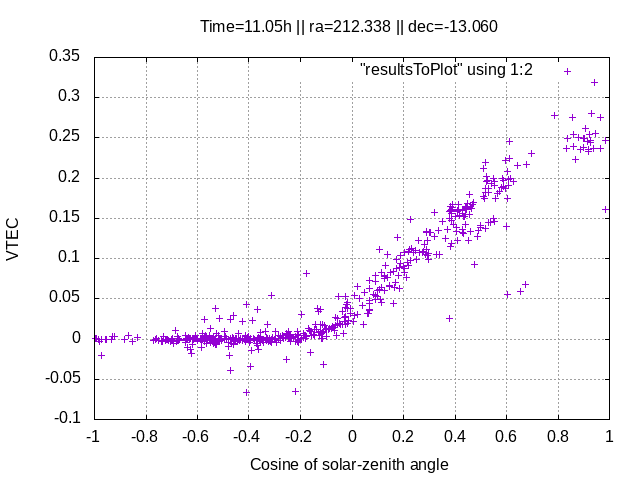
\includegraphics[width=0.5\linewidth]{images/ch4/resultSunTest.png}
	\caption{VTEC value as a function of the solar-zenith angle cosine}
	\label{fig:results}
\end{centering}
\end{figure}

As we can observe, the resulting plot, similar to the one from figure \ref{fig:halloweenPaper}, shows a strong relation between the cosine of the solar-zenith angle and the VTEC content, which increases from $\cos\chi = 0$ (90º) to $\cos\chi = 1$ (0º) and it doesn't seem to affect it from $\cos\chi = -1$ (180º) to $\cos\chi = 1$ (0º). \\

Visually this can be seen as follows:

\begin{figure}[!htb]
	\begin{centering}
		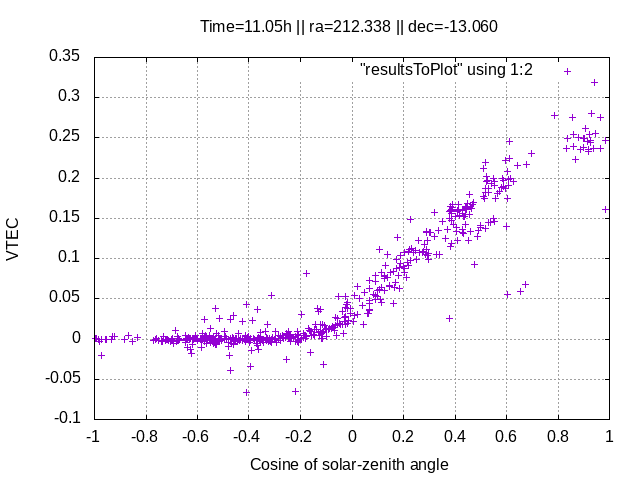
\includegraphics[width=0.5\linewidth]{images/ch4/resultSunTest.png}
		\caption{VTEC value as a function of the solar-zenith angle cosine}
		\label{fig:comparison}
	\end{centering}
\end{figure}

When the Sun is vertically on the sun





In conclusion, we can see that there appears to be correlation between the two variables. This correlation will be studied in more detail in the following section, where a first approach of the algorithm will be presented to detect the flare without knowing its location.













